\chapter{Methodology}\label{C:Methodology}

This chapter outlines the methodology that was followed to obtain findings in this study. The methodology is then further deconstructed to describe the data collection and data analysis process. The data collection subsection provides a summary of the participants.

\section{Grounded Theory} 

Grounded Theory (GT) is the chosen methodology for this study. This was an appropriate choice as the study focuses on human aspects, and GT is a way of analysing qualitative data with the end-goal of defining a new theory from the sampled data \cite{geeks}. There are several steps in the GT  methodology in order to make the final theory.  The theory is expected to be explanatory, focusing on describing elements of the findings rather than stating. The theory should also be based on the collected responses and observations, rather than pre-conceived ideas. As such, extensive literature reviews should be avoided.
\newline
\par Initially, researchers must choose a topic and determine whether the Grounded Theory method is the right one for the research project \cite{geeks}. After contacting potential participants, an iterative process of data collection occurs. Questions adapt between the rounds of the collection as the data is analysed. This refinement of questions happens to delve deeper into the traits of the emerging theory. When saturation is achieved, no further new findings are displayed which contribute to the final theory. This results in the “grounded” nature of the overall theory.
\newline
\par 
In the study outlined in this report, at approximately ten interviews, the concepts obtained from the data collection started to become quite similar. This is called saturation point and is when some new lower-level ideas are being obtained, but no overly new information. This was the grounding point of this specific Grounded Theory. 
\newline

\begin{figure}[ht]
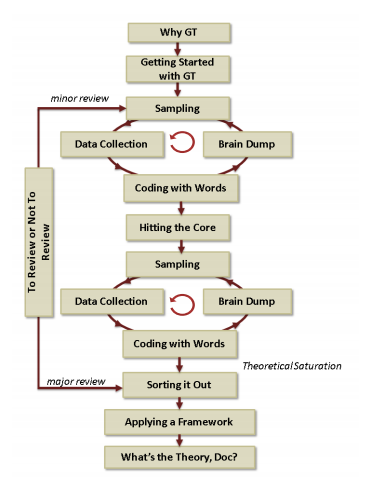
\includegraphics[width=8cm]{figures/fig1.png}
\centering
\caption{The Grounded Theory Pattern (Hoda, Noble, \& Marshall, 2011) Used with Permission \cite{geeks}}
\centering
\end{figure}

\par Initially, I aimed to get more technical empirical evidence on programmers and their security practices. I, however, identified as early as the third interview that technical security programming practices are not as influential as initially thought, and the interview questions changed to match this gradual shift in focus. This is another benefit of Grounded Theory as questions do not have to stay the same; instead, they undergo iterations of development as an area of interest shifts.  


\section{Data Collection} 

\subsection{Recruitment}
\par A recruitment post and webpage was sent to mailing lists and websites like OWASP Meetup and LinkedIn \cite{webpage}. These are shown in Appendix E and Appendix F, respectively. There was a brief halt in the recruiting through the Meetup website as I got banned for posting in groups as I was marked as spam. However, I did not get much interest from the promotion through both Meetup and Linkedin and instead relied on personal contacts (friends and family-friends) and supervisor contacts for initial recruitment. Participants also helped with recruitment by reaching out to others in the industry and telling them about this study. 

\subsection{Interviews}

\par Fifteen interviews were conducted with participants across New Zealand. These participants were from fourteen unique organisations. Participants had varying job titles, years of experience, and were in a range of different sectors and organisation fields. The diversity within the participants allowed for connections to be made across a broader range of people. 
\newline
\par Human Ethics approval had to be gained before the interview process could commence (Appendix B). Initial questions were developed based on a small pilot study run on two recent graduates of the School of Engineering at Victoria University of Wellington. Overall, this small pilot study was essential in providing some more clarity on the interview process. It also supplied practice in conducting interviews and has helped in the continuous process of defining questions.
\newline
\par After Human Ethics had been approved the interview process started. Questions were adapted dependent on the analysis between the interviews and changed as a result of participants answers within the interview. This was so any intriguing information could be queried further during the semi-structured interview. Therefore, the list of interview questions in Appendix D changed with only the "Participant Background" section remaining as a constant.
\newline
\par Due to the disruptive year, interviews were predominantly conducted over Zoom. Consent from the participants was obtained through an email response as per Human Ethics committee request. Interviews ran for periods ranging between 30-90 minutes. A summary of the participant sample is provided in the table below. 
\newline
\newline

\begin{table}[!hb]
\begin{tabular}{|l|l|l|}
\hline
\multicolumn{1}{|c|}{\textbf{Alias}} & \multicolumn{1}{|c|}{\textbf{Role}}                           & \multicolumn{1}{|c|}{\textbf{Experience (Years)}} \\ \hline
\multicolumn{1}{|l|}{P1}           & \multicolumn{1}{l|}{Enterprise Architect and Domain Lead}   & \multicolumn{1}{l|}{15\textless{}}             \\ \hline
\multicolumn{1}{|l|}{P2}           & \multicolumn{1}{l|}{Principal Product Architect}            & \multicolumn{1}{l|}{15\textless{}}             \\ \hline
\multicolumn{1}{|l|}{P3}           & \multicolumn{1}{l|}{Senior Security Architect}              & \multicolumn{1}{l|}{10-15}                      \\ \hline
\multicolumn{1}{|l|}{P4}           & \multicolumn{1}{l|}{Senior Software Engineer}               & \multicolumn{1}{l|}{15\textless{}}              \\ \hline
\multicolumn{1}{|l|}{P5}           & \multicolumn{1}{l|}{Software Developer}                     & \multicolumn{1}{l|}{\textless 2}                \\ \hline
\multicolumn{1}{|l|}{P6}           & \multicolumn{1}{l|}{Level 2 Security Analyst}               & \multicolumn{1}{l|}{2-5}                        \\ \hline
\multicolumn{1}{|l|}{P7}           & \multicolumn{1}{l|}{Site Reliability Engineer}              & \multicolumn{1}{l|}{\textless 2}                \\ \hline
\multicolumn{1}{|l|}{P8}           & \multicolumn{1}{l|}{DevOps Engineer}                        & \multicolumn{1}{l|}{\textless 2}                \\ \hline
\multicolumn{1}{|l|}{P9}           & \multicolumn{1}{l|}{Portfolio Architect}                    & \multicolumn{1}{l|}{10-15}                      \\ \hline
\multicolumn{1}{|l|}{P10}          & \multicolumn{1}{l|}{Full-stack Software Developer}          & \multicolumn{1}{l|}{2-5}                        \\ \hline
\multicolumn{1}{|l|}{P11}          & \multicolumn{1}{l|}{Cloud Engineer}                         & \multicolumn{1}{l|}{2-5}                        \\ \hline
\multicolumn{1}{|l|}{P12}          & \multicolumn{1}{l|}{Consultant (Cloud Engineering)}         & \multicolumn{1}{l|}{2-5}                        \\ \hline
\multicolumn{1}{|l|}{P13}          & \multicolumn{1}{l|}{Development Manager and Technical Lead} & \multicolumn{1}{l|}{10-15}                      \\ \hline
\multicolumn{1}{|l|}{P14}          & \multicolumn{1}{l|}{Senior Software Engineer}               & \multicolumn{1}{l|}{10-15}                      \\ \hline
P15                                & Business Rule Consultant                                    & 15\textless{}                                   \\ \hline
\end{tabular}
\centering
\caption{Participant Aliases and Summary}
\centering
\end{table}

\section{Data Analysis} 

After transcribing interviews and pairing them with written observations), the selective coding process occurs \cite{geeks}. Key points from each transcript are paired with a simplified summary of the points \cite{geeks}. The constant comparison method is used where codes are compared to others from within the same interview and also with other interviews \cite{geeks}. These comparisons continue to occur, and are further narrowed to become categories for the theory \cite{geeks}, also referred to as selective coding \cite{geeks}. Therefore, this coding process has three key steps. Theoretical notes are written throughout this coding process to research relationships between concepts and categories \cite{geeks}. An emergent theory is then formed which aims to explain a practice or a phenomenon. 








